\documentclass{article}


\usepackage{graphicx}

\begin{document}

\title{Dependent services}

\maketitle


\section{Experiment Design}

Suppose the services have dependencies between each other, e.g., to provide service 1, you must first provide service 2, 3. Any platform must satisfy the service dependencies, but the applications do not need to explicitly specify the required services and all their dependencies. 

This is an analog to the Eclipse platforms and their plugins.

\section{Implementation}

\begin{itemize}
\item
\texttt{ServiceDependencies}: A class to generate dependencies between services, as a DAG
\item
\texttt{MutualisticGraph} (modified): When creating platforms, it makes sure that all to satisfy the dependency.

\end{itemize}

\section{Configuration}
\texttt{Configuration::NDEP}: How may links to create between services


\section{Results}



\begin{figure}
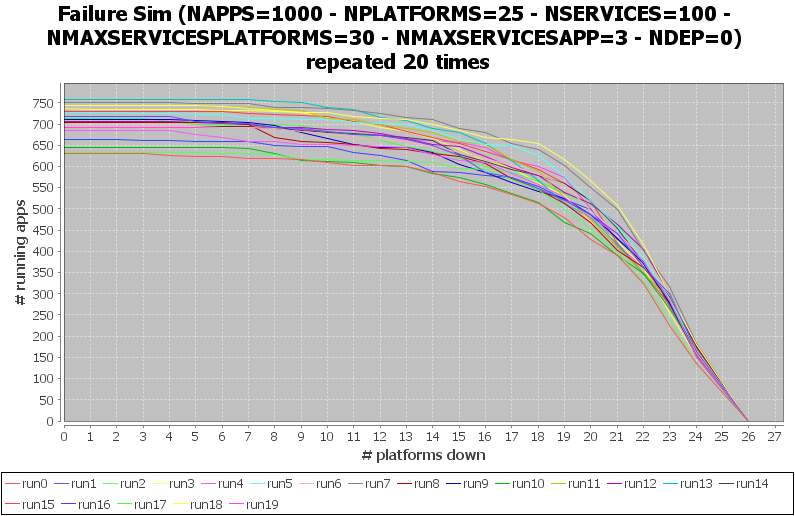
\includegraphics[width=1.0\textwidth]{dep0}
\caption{NDEP=0: Same as original experiment}
\end{figure}


\begin{figure}
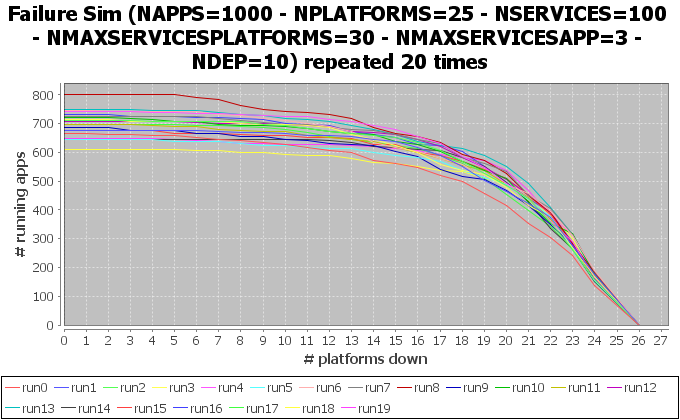
\includegraphics[width=1.0\textwidth]{dep10}
\caption{NDEP=10:  it seems that that the curve goes down a bit more quickly (not very sure...)}
\end{figure}

\begin{figure}
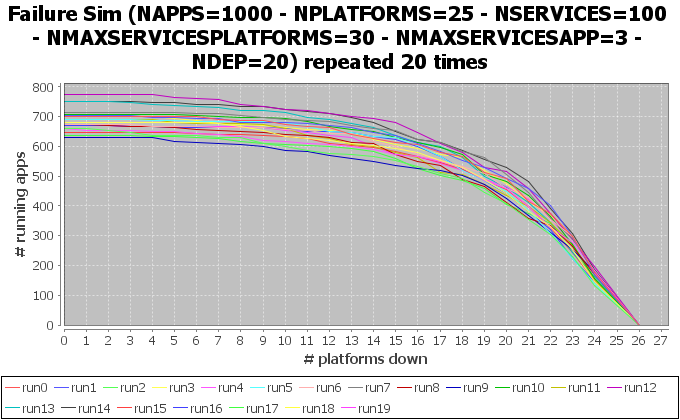
\includegraphics[width=1.0\textwidth]{dep20}
\caption{NDEP=20:  similar trend?}
\end{figure}

\begin{figure}
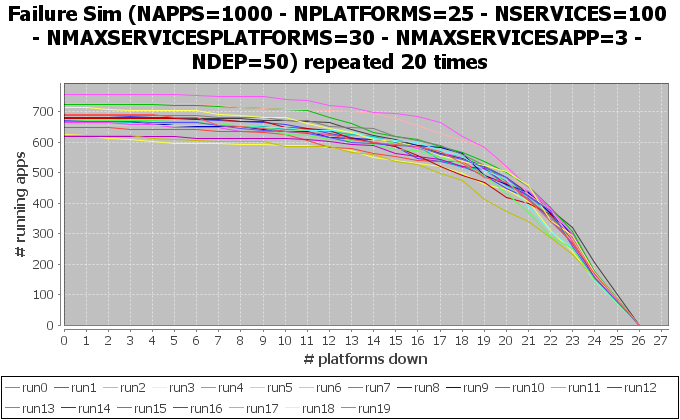
\includegraphics[width=1.0\textwidth]{dep50}
\caption{NDEP=50:  from smooth curve to staircase curve. Probably because the platforms are homogenized}
\end{figure}

\begin{figure}
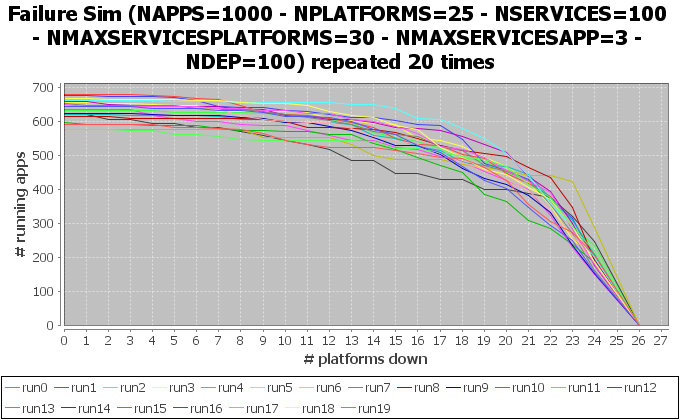
\includegraphics[width=1.0\textwidth]{dep100}
\caption{NDEP=100: staircase curve}
\end{figure}

\begin{figure}
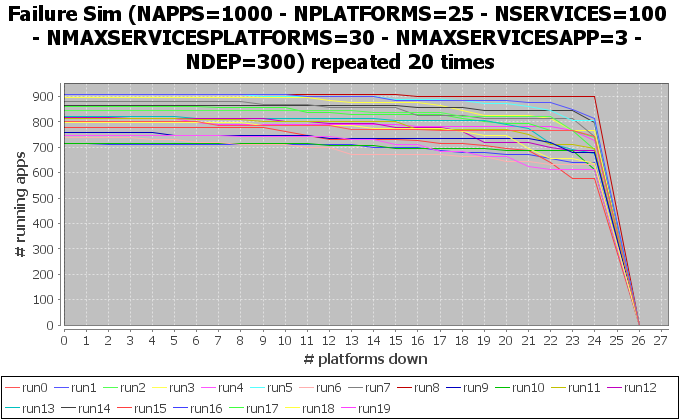
\includegraphics[width=1.0\textwidth]{dep300}
\caption{NDEP=300: super staircase curve}
\end{figure}



\begin{figure}
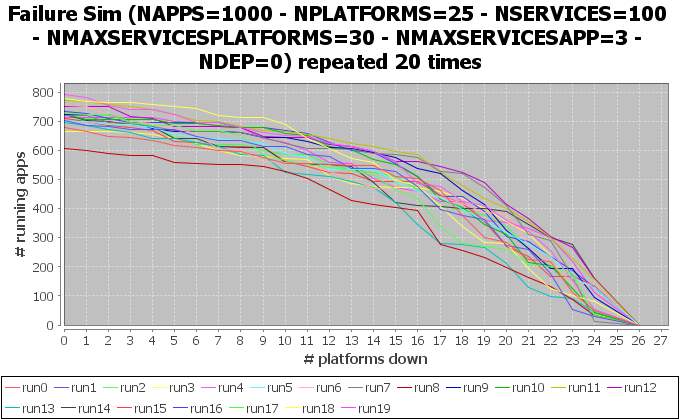
\includegraphics[width=1.0\textwidth]{dep0-noorder}
\caption{NDEP=0, kill platforms in the same order as they are created: slightly staircase curve(?)}
\end{figure}

\begin{figure}
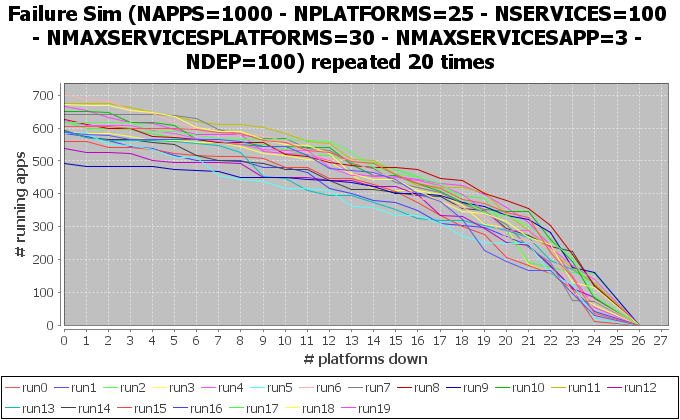
\includegraphics[width=1.0\textwidth]{dep100-noorder}
\caption{NDEP=300, kill platforms in the same order as they are created: no big difference}
\end{figure}

\begin{figure}
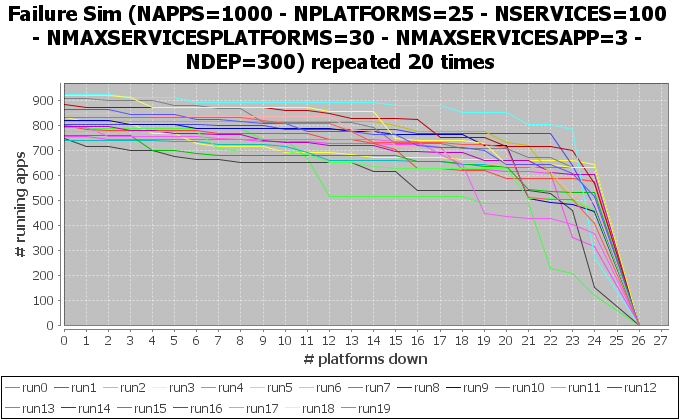
\includegraphics[width=1.0\textwidth]{dep300-noorder}
\caption{NDEP=300, kill platforms in the same order as they are created: super staircase curve}
\end{figure}

\section{Discussion}

It seems that currently the results are not obvious at all, and the trend is not coherent! We will try to see if changing the configurations of platform/service/app numbers or use different way to kill platforms will make some more interesting results.

\end{document}